\documentclass{standalone}
\usepackage{tikz}
\usetikzlibrary{calc}
\usetikzlibrary{arrows.meta}


\begin{document}
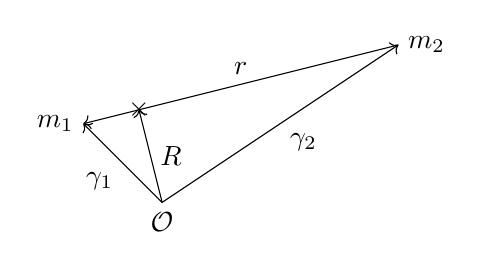
\begin{tikzpicture}
	\coordinate (origin)	at (0,0);
	\coordinate (mass1)		at (-1,1);
	\coordinate (mass2)		at (3,2);
%	\filldraw (mass1) circle (2pt);
%	\filldraw (mass2) circle (2pt);

 	\node[below]	()	at (origin)	{$\mathcal{O}$};
	\node[left]		()	at (mass1)	{$m_1$};
	\node[right]	()	at (mass2)	{$m_2$};
	
	\draw[->, anchor=south] (origin) -- (mass1) node[below left, pos = .5] {$\gamma_1$};
	\draw[->, anchor=south] (origin) -- (mass2) node[below right,pos = .5] {$\gamma_2$};
	\draw[->] (mass2) -- (mass1) node[above, pos = .5] {$r$};
	\draw[->] (origin) -- ($(mass1)!(origin)!(mass2)$) node[right,pos = 0.5] {$R$} node {$\times$};
\end{tikzpicture}

\end{document}